
\section{Problem Statement}
My team at Statcon Electronics India Ltd has been focusing on enhancing the
efficiency and performance of Switched Mode Power Supplies. Presently, most
SMPS utilize switching of MOSFETs at high frequencies to generate an alternating
high frequency signal which is then passed through a rectifier and filtered using
capacitors. We use LLC Based Resonant Converters which have higher efficiency, and
lower output voltage ripple than traditional SMPS. The aim of this project is to
understand the working of such a converter and design one as well

\section{Overview}

\subsection{LLC Converter}
Figure \ref{fig:llc_converter} is a schematic of a basic LLC converter. The LLC has the
following components:

\begin{figure}[h]
    \centering
    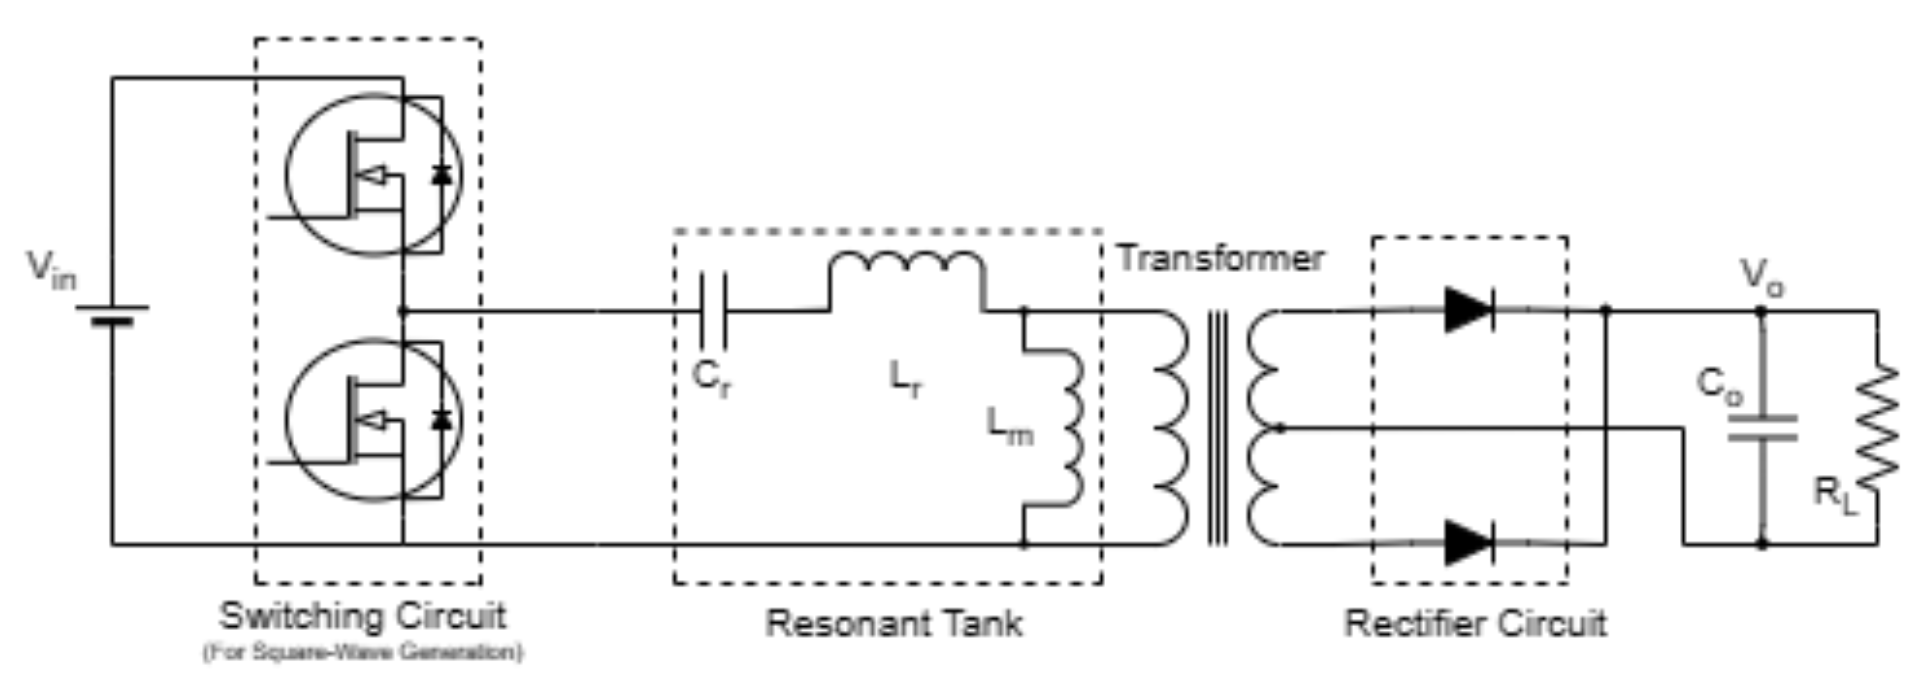
\includegraphics[width=\textwidth]{LLC_converter.png}
    \caption{Diagram of an LLC based resonant converter}
    \label{fig:llc_converter}
\end{figure}

\noindent

\subsubsection{Switching Circuit}
The switching circuit alternately switches the MOSFETs ON and OFF (full-bridge or half-bridge), generating a sort of square wave after the switching circuit, and before the resonant tank circuit.
\subsubsection{Resonant Tank}
The resonant tank circuit filters the higher-order harmonics and generates a sinusoidal signal of the fundamental frequency of the tank circuit to be fed into the primary side of the transformer.
\subsubsection{Rectifier Circuit}
A bridge rectifier (full-bridge or half-bridge) followed by the output capacitor rectifies the alternating voltage produced at the transformer and converts it into stable DC voltage.

\section{Challenges}
The challenges I faced in simulating and designing a LLC Based Resonant converter include:
\begin{itemize}
    \item \textbf{Modeling the LLC converter}: Understanding the complex interactions between the switching circuit, resonant tank, and rectifier circuit and accurately modeling their behavior in simulation.
    \item \textbf{Component selection}: Choosing the appropriate resonant tank components to ensure optimal performance and efficiency.
    \item \textbf{Efficiency optimization}: Optimizing the converter design to maximize efficiency and minimize power losses.
    \item \textbf{Cost considerations}: Balancing the performance requirements with cost constraints to design a converter that is both efficient and cost-effective.
    \item \textbf{Validation and testing}: Verifying the performance of the designed converter through simulation and experimental testing to ensure it meets the desired specifications.
    \item \textbf{Load Sharing}: The biggest challenge was when we hooked up multiple LLCs in parallel to perform load sharing and we observed oscillications in the load shared. This was solved later by my analysis of the circuit.
\end{itemize}